\chapter{扩展:改进Poisson求解器}
\label{ch:poisson}


\begin{quote}
我们迄今为止撰写的FENICS计划已经设计为平面设计
Python脚本。 这对于解决简单的演示非常有用
问题。 但是,当您构建高级的求解器时
应用程序,你会很快找到需要更多的结构化
节目。 特别是,您可能希望重用您的求解器来解决
大量的问题,你们改变边界条件,
域,以及材料参数等系数。 在本章中,
我们将看到如何编写一般的求解器函数来改进
FEniCS计划的可用性。 我们也会讨论如何
利用具有预处理器的迭代求解器来求解线性
系统,如何计算派生数量,例如通量
在边界的一部分,以及如何计算错误和收敛
率。
\end{quote}

\section{重构Poisson求解器}
\label{ch:poisson0:impl2}

\index{flat program}

本书中讨论的大多数程序是“平”就是他们是
在Python方面没有组织成逻辑,可重复使用的单位
功能。这样的平面程序对于快速测试想法是有用的
素描解算法,但不适合严重
解决问题因此,我们将看看如何\emph{refactor}
Poisson求解器从Chapter~\ref{ch:fundamentals}。一开始就这样
意味着将代码分解为函数。但重构不仅仅是一个
重新排列现有声明。在重构期间,我们也尝试
使我们创建的功能尽可能在其他方面可重用
上下文。我们也会封装一些具体的陈述
问题变成(不可重用)的功能。能够区分
当重构时,专用代码的可重用代码是一个关键问题
代码,这个能力取决于一个很好的数学理解
手头的问题(什么是一般的,什么是特殊的)。在一个单位
程序,一般和专门的代码(和数学)经常
混合在一起,这往往会给人一种模糊的理解
手头的问题。

\subsection{更一般的求解器函数}
\label{ch:poisson0:impl2:func}

我们考虑平面计划
\url{{https://fenicsproject.org/pub/tutorial/python/vol1/ft01_poisson.py}}{\nolinkurl{ft01_poisson.py}}
解决了Poisson问题的开发
在章节~\ref{ch:fundamentals}。
这个程序中的一些代码
需要解决任何Poisson问题$-\nabla^2 u=f$ on $[0,1]\times
[0,1]$与$u=\ub$在边界上,而其他语句来自
我们简单的测试问题。 让我们收集一般的,可重复使用的代码
一个名为\texttt{solver}的函数。 我们的特殊测试问题就是这样
我们的\texttt{solver}的一个应用程序附加了一些其他语句。 我们限制
\texttt{solver}函数来计算数值
解。 绘制和比较解决方案与确切的解决方案
被认为是要执行的特定于问题的活动
别处。

我们将\texttt{solver}参数化为$f$, $\ub$和分辨率
目。 因为使用高阶有限元是如此微不足道
函数通过将第三个参数改为\texttt{FunctionSpace},我们
还加入有限元函数空间的多项式度
作为\texttt{solver}的参数。

\begin{python}
from fenics import *
import numpy as np

def solver(f, u_D, Nx, Ny, degree=1):
    """
    Solve -Laplace(u) = f on [0,1] x [0,1] with 2*Nx*Ny Lagrange
    elements of specified degree and u = u_D (Expresssion) on
    the boundary.
    """

    # Create mesh and define function space
    mesh = UnitSquareMesh(Nx, Ny)
    V = FunctionSpace(mesh, 'P', degree)

    # Define boundary condition
    def boundary(x, on_boundary):
        return on_boundary

    bc = DirichletBC(V, u_D, boundary)

    # Define variational problem
    u = TrialFunction(V)
    v = TestFunction(V)
    a = dot(grad(u), grad(v))*dx
    L = f*v*dx

    # Compute solution
    u = Function(V)
    solve(a == L, u, bc)

    return u
\end{python}

我们的初始程序的其余任务,如调用\texttt{solver}
功能与问题特定的参数和绘图,
可以放在一个单独的功能。 这里我们选择放这个代码
在一个名为\verb!run_solver!的函数中:

\begin{python}
def run_solver():
    "Run solver to compute and post-process solution"

    # Set up problem parameters and call solver
    u_D = Expression('1 + x[0]*x[0] + 2*x[1]*x[1]', degree=2)
    f = Constant(-6.0)
    u = solver(f, u_D, 8, 8, 1)

    # Plot solution and mesh
    plot(u)
    plot(u.function_space().mesh())

    # Save solution to file in VTK format
    vtkfile = File('poisson_solver/solution.pvd')
    vtkfile << u
\end{python}

该解决方案现在可以被计算,绘制和保存到文件
只需调用\verb!run_solver! 功能。

\subsection{将求解器写为Python模块}

\index{Python module}

重构的代码放在一个文件中
\url{{https://fenicsproject.org/pub/tutorial/python/vol1/ft12_poisson_solver.py}}{\nolinkurl{ft12_poisson_solver.py}}。
我们应该确保这样的文件可以导入(因此
重用)在其他程序。 这意味着所有的语句在主
不在功能内的程序应该出现在测试中
\verb!if __name__ == '__main__':! 如果文件被执行,则该测试是真实的
一个程序,但是假的如果导入文件。 如果我们想运行这个
文件的方式与我们可以运行\verb!ft01_poisson.py!,相同
主程序只是一个调用\verb!run_solver! 其次是电话
\texttt{interactive}保存情节:

\begin{python}
if __name__ == '__main__':
    run_solver()
    interactive()
\end{python}
这个完整的程序可以在文件中找到\url{{https://fenicsproject.org/pub/tutorial/python/vol1/ft12_poisson_solver.py}}{\nolinkurl{ft12_poisson_solver.py}}。

\index{ft12\_poisson\_solver.py@{\rm\texttt{ft12\_poisson\_solver.py}}}
\index{unit testing}

\subsection{验证和单元测试}

\index{verification}

我们的第一个程序的剩余部分是比较数字
和确切的解决方案。 每次我们编辑代码,我们必须重新运行
测试并检查\verb!error_max! 足够小,所以我们知道
该代码仍然有效。 为此,我们将采用单元测试,
意味着我们创建了一个数学测试和相应的软件
可以自动运行所有测试,并检查所有测试
通过。 Python有几个单元测试工具。 两个很受欢迎
一个是pytest和nose。 这几乎是一样的,非常容易
使用。 通过测试类提供更经典的单元测试
内置模块\texttt{unittest},但是这里我们要使用pytest
(或nose),因为这将导致更短和更清晰的代码。

在数学上,我们的单元测试是有限元解
我们的问题当$f=-6$等于确切的解决方案$u=\ub=1+x^2+2y^2$
在网格的顶点。
我们已经创建了一个在顶点找到错误的代码
我们的数值解。 由于四舍五入的错误,我们不能要求这个
错误为零,但是我们必须使用一个容差,哪个
取决于元素的数量和多项式的程度
在有限元的基础上。 如果我们要测试那个
\texttt{solver}函数适用于高达$2\times(20\times 20)$的网格
元素和立方体Lagrange元素,$10^{-10}$是适当的
容忍测试最大误差消失。

为了使我们的测试用例与pytest和nose一起工作,我们必须
对我们的程序进行几个小的调整。 简单
规则是每个测试都必须放在一个函数中

\begin{itemize}
 \item 名字以\verb!test_!开头

 \item 没有论据,

 \item 执行表示为\texttt{assert success, msg}的测试。
\end{itemize}

\noindent
关于最后一点,\texttt{success}是一个布尔表达式
\texttt{False}如果测试失败,在这种情况下,字符串\texttt{msg}是
写入屏幕。 当测试失败时,\texttt{assert}会引发一个
Python中的\texttt{AssertionError}异常,否则运行
默默。 \texttt{msg}字符串是可选的,所以\texttt{assert success}是
最小测试。 在我们的例子中,我们会写\verb!assert error_max <tol!,
其中\texttt{tol}是上述容限。

在该单元测试中执行适当的测试功能
pytest或nose测试框架具有以下形式。 注意
我们对不同的网格分辨率和度数执行测试
有限元。

\begin{python}
def test_solver():
    "Test solver by reproducing u = 1 + x^2 + 2y^2"

    # Set up parameters for testing
    tol = 1E-10
    u_D = Expression('1 + x[0]*x[0] + 2*x[1]*x[1]', degree=2)
    f = Constant(-6.0)

    # Iterate over mesh sizes and degrees
    for Nx, Ny in [(3, 3), (3, 5), (5, 3), (20, 20)]:
        for degree in 1, 2, 3:
            print('Solving on a 2 x (%d x %d) mesh with P%d elements.'
                  % (Nx, Ny, degree))

            # Compute solution
            u = solver(f, u_D, Nx, Ny, degree)

            # Extract the mesh
            mesh = u.function_space().mesh()

            # Compute maximum error at vertices
            vertex_values_u_D = u_D.compute_vertex_values(mesh)
            vertex_values_u  = u.compute_vertex_values(mesh)
            error_max = np.max(np.abs(vertex_values_u_D - \
                                      vertex_values_u))

            # Check maximum error
            msg = 'error_max = %g' % error_max
            assert error_max < tol, msg
\end{python}

要运行测试,我们键入以下命令:

\begin{bash}
$ py.test ft12_poisson_solver.py
\end{bash}
这将运行所有名为\verb!test_ *!的函数(目前只有
\verb!test_solver!函数)在文件中找到并报告结果。
对于更详细的输出,请添加flags \texttt{-s -v}。

我们将会习惯于将数字测试问题包含进来
单元测试如上,我们强烈鼓励读者创建
每当实施FEniCS求解器时,进行类似的单元测试。

\begin{notice}[提示:在测试功能中打印消息]
当测试通过时,\texttt{assert}语句静默运行,以便用户可以
测试功能中的所有语句是否真的会变得不确定
执行。 心理帮助是在\texttt{assert}之前打印出一些东西
(正如我们在上面的例子中所做的那样),这样很清楚
测试真的发生了。
请注意,\texttt{py.test}需要\texttt{-s}选项来显示打印输出
从测试功能。
\end{notice}

\begin{notice}[提示:使用iPython进行调试]
可以通过添加以下内容从Python脚本轻松输入iPython
代码中的任何位置:
\begin{python}
from IPython import embed; embed()
\end{python}
这一行开始一个交互式的Python会话,让你
打印和绘图变量,这对调试非常有帮助。
\end{notice}

\subsection{参数化空间维数}
\label{ch:poisson0:nD}
\index{dimension-independent code}

\index{space dimensions}

FEniCS可以很容易地编写一个可以统一的模拟代码
操作在1D,2D和3D。 作为开胃菜,回到
以前的节目
\url{{https://fenicsproject.org/pub/tutorial/python/vol1/ft01_poisson.py}}{\nolinkurl{ft01_poisson.py}}
要么
\url{{https://fenicsproject.org/pub/tutorial/python/vol1/ft12_poisson_solver.py}}{\nolinkurl{ft12_poisson_solver.py}}
并将网格构造从\texttt{UnitSquareMesh(8,8)}更改为
\texttt{UnitCubeMesh(8,8,8)}。 现在域是单位立方体
分为$8\times 8\times 8$
盒子和每个盒子
分为六个四面体形有限元
计算。 运行程序,观察我们可以解决3D
问题没有任何其他修改! (在1D中,表达式必须是
修改为不依赖于\texttt{x [1]})。可视化允许你
旋转立方体并观察功能值作为颜色
边界。

如果我们要参数化单位间隔的创建,单位平方,
或单位立方体尺寸,我们可以通过封装这部分来实现
的函数中的代码。 给定一个列表或元组指定除法
进入空格坐标中的单元格,具有以下功能
返回$d$维数多维数据集的网格:

\begin{python}
def UnitHyperCube(divisions):
    mesh_classes = [UnitIntervalMesh, UnitSquareMesh, UnitCubeMesh]
    d = len(divisions)
    mesh = mesh_classes[d - 1](*divisions)
    return mesh
\end{python}
施工\verb!mesh_class[d - 1]! 会选出正确的名字
用于定义域并生成网格的对象。 而且,
参数\texttt{* divisions}发送列表的所有组件\texttt{divisions}
作为网格构造的构造函数的单独参数
类由\verb!mesh_class[d - 1]!挑选出来。 例如,在2D问题中
其中\texttt{divisions}有两个元素,即语句

\begin{python}
mesh = mesh_classes[d - 1](*divisions)
\end{python}
相当于

\begin{python}
mesh = UnitSquareMesh(divisions[0], divisions[1])
\end{python}

\texttt{solver}函数
\url{{https://fenicsproject.org/pub/tutorial/python/vol1/ft12_poisson_solver.py}}{\nolinkurl{ft12_poisson_solver.py}}
可以通过替换来修改$d$维度问题
\texttt{Nx}和\texttt{Ny}参数由\texttt{divisions}调用,并调用该函数
\texttt{UnitHyperCube}创建网格。 注意\texttt{UnitHyperCube}是一个
\emph{function}而不是\emph{class},但是我们使用所谓的命名它
\emph{CamelCase符号}使其看起来像一个类:

\begin{python}
mesh = UnitHyperCube(divisions)
\end{python}

\section{使用线性求解器}
\label{ch:poisson0:solve:prm}

默认使用稀疏LU分解(Gaussian消除)
在FEniCS程序中求解线性方程组。 这是非常
鲁棒简单的方法。 这是系统的推荐方法
最多有几千个未知数,因此可能是其中的一种
许多2D和更小的3D问题的选择。 但是,稀疏LU
分解变慢,一个快速耗尽内存
更大的问题 对于大问题,我们需要使用\emph{iterative
方法}它们更快,需要更少的内存。 我们现在
看看如何利用最先进的迭代解决方案
FEniCS中的方法。

\subsection{选择线性求解器和预处理器}

\index{linear solver}
\index{preconditioner}
\index{Krylov solver}

预处理Krylov求解器是一种流行的迭代方法
在FEniCS程序中可以轻松访问。 Poisson方程
产生一个对称的正定系统矩阵,为此,
最优Krylov求解器是Conjugate Gradient(CG)方法。 对于
非对称问题,非对称系统的Krylov求解器,
如GMRES,是一个更好的选择。 不完整LU分解(ILU)
是一个流行和强大的全面预处理器,所以让我们试试
GMRES-ILU对:

\begin{python}
solve(a == L, u, bc,
      solver_parameters={'linear_solver': 'gmres',
                         'preconditioner': 'ilu'})
# Alternative syntax
solve(a == L, u, bc,
      solver_parameters=dict(linear_solver='gmres',
                             preconditioner='ilu'))
\end{python}
部分~\ref{ftut:app:solver:prec}列出了最受欢迎的选择
Krylov解决方案和预处理器可用于FEniCS。

\index{linear algebra backend}
\index{PETSc} \index{Eigen}

\subsection{选择线性代数后端}

实际的GMRES和ILU实施被采取行动
取决于线性代数包的选择。 FEniCS接口
几个线性代数包,称为\emph{linear algebra backends}
FEniCS术语。 如果FEniCS被编译,PETSc是默认选择
与PETSc。 如果PETSc不可用,则FEniCS将回退使用
Eigen后端。 FEniCS中的线性代数后端可以设置
使用以下命令:

\begin{python}
parameters.linear_algebra_backend = backendname
\end{python}
\texttt{backendname}是一个字符串。 查看哪个线性代数后端
可用,您可以调用FEniCS功能
\verb!list_linear_algebra_backends! 同样,可以查看哪一个
线性代数后端正在被以下使用
命令:

\begin{python}
print(parameters.linear_algebra_backend)
\end{python}

\index{parameters@{\rm\texttt{parameters}}}
\index{info@{\rm\texttt{info}}}

\subsection{设置求解器参数}

我们通常会在停止时控制容差
标准和运行时的最大迭代次数
迭代法 这样的参数可以在全局控制
和地方一级。 我们将从如何设定全球化开始
参数。 对于更高级的程序,可能需要使用一个数字
的不同线性求解器并设置不同的公差等
参数。 那么在a处控制参数变得很重要
地方一级。 我们将在~\ref{ch:poisson0:solver:problem}部分中回到此问题。

更改全局FEniCS参数数据库中的参数会影响
所有线性求解器(在参数设置后创建)。
全局FEniCS参数数据库简称为\texttt{parameters}和
它表现为一个嵌套字典。 写

\begin{python}
info(parameters, verbose=True)
\end{python}
列出数据库中的所有参数及其默认值。
参数集的嵌套通过缩进表示
从\texttt{info}输出。
根据该输出,相关参数集为
命名为\verb!'krylov_solver'!,参数设置如下:

\begin{python}
prm = parameters.krylov_solver  # short form
prm.absolute_tolerance = 1E-10
prm.relative_tolerance = 1E-6
prm.maximum_iterations = 1000
\end{python}
针对Krylov求解器的停止标准通常涉及一些规范
剩余值必须小于绝对公差
参数或小于相对公差参数次数
初始残留。

我们注意到,全局参数数据库的默认值可以是
在XML文件中定义。 从当前集合生成这样的文件
的程序中的参数,运行

\begin{python}
File('parameters.xml') << parameters
\end{python}
如果一个\verb!dolfin_parameters.xml! 文件在目录中找到
运行FEniCS程序,该文件被读取并用于初始化
\texttt{parameters}对象。 否则,该文件
\verb!.config/fenics/dolfin_parameters.xml!
在用户的主目录是
阅读,如果存在。 另一个选择是加载XML文件(与任何
名称)手动在程序中:

\begin{python}
File('parameters.xml') >> parameters
\end{python}
XML文件也可以是gzip的形式,扩展名为\texttt{.xml.gz}。

\subsection{扩展求解器函数}

我们可能会扩展以前的求解器函数
\url{{https://fenicsproject.org/pub/tutorial/python/vol1/ft12_poisson_solver.py}} {\nolinkurl{ft12_poisson_solver.py}}
在部分〜\ref{ch:poisson0:impl2:func}
这样它也提供了GMRES + ILU
预处理Krylov求解器:

\index{ft10\_poisson\_extended.py@{\rm\texttt{ft10\_poisson\_extended.py}}}

这个新的\texttt{solver}函数在文件中找到
\url{{https://fenicsproject.org/pub/tutorial/python/vol1/ft10_poisson_extended.py}} {\nolinkurl{ft10_poisson_extended.py}},
取而代之
\url{https://fenicsproject.org/pub/tutorial/python/vol1/ft12_poisson_solver.py} {\nolinkurl{ft12_poisson_solver.py}}。
它具有以前\texttt{solver}功能的所有功能,但是
也可以用迭代法解决线性系统。

subsection{关于单元测试的评论}

关于以单位来验证新的\texttt{solver}函数
测试,事实证明单位测试的问题在哪里
当我们使用时,近似误差消失会变得更加复杂
迭代方法。问题是由于迭代而保持错误
解决方案小于验证中使用的公差
试验。首先,这意味着Krylov中使用的公差
求解器必须小于\texttt{assert}测试中使用的公差,
但是这并不能保证线性求解误差小。
对于线性元素和小网格,容差为$10^{-11}$作品
在Krylov求解器的情况下(使用容限$10^{-12}$)
在那些解答者)。有兴趣的读者参考
\verb!demo_solvers!功能在
\url{https://fenicsproject.org/pub/tutorial/python/vol1/ft10_poisson_extended.py} {\nolinkurl{ft10_poisson_extended.py}}
详情请见:
该函数测试直接和迭代的数值解
线性求解器,适用于不同网格,不同程度的
有限元基函数中的多项式。

\subsection{线性求解器方法和预处理器列表}
\label{ftut:app:solver:prec}

\index{linear solver}
\index{Krylov solver}
\index{preconditioner}

哪些线性求解器和预处理器可用
在FEniCS中取决于FEniCS的配置以及哪些
线性代数后端当前处于活动状态。 下表
显示了可用的线性求解器的示例
当PETSc后端处于活动状态时,通过FEniCS:

{\small

\vspace{4mm}

\begin{tabular}{ll}
\hline\noalign{\smallskip}
\multicolumn{1}{c}{ 名称 } & \multicolumn{1}{c}{ 方法 } \\
\noalign{\smallskip}\hline\noalign{\smallskip}
\texttt{'bicgstab'}     & Biconjugate gradient stabilized method       \\
\texttt{'cg'}           & Conjugate gradient method                    \\
\texttt{'gmres'}        & Generalized minimal residual method          \\
\texttt{'minres'}       & Minimal residual method                      \\
\texttt{'petsc'}        & PETSc built in LU solver                     \\
\texttt{'richardson'}   & Richardson method                            \\
\verb!'superlu_dist'! & Parallel SuperLU                             \\
\texttt{'tfqmr'}        & Transpose-free quasi-minimal residual method \\
\texttt{'umfpack'}      & UMFPACK                                      \\
\noalign{\smallskip}\hline\noalign{\smallskip}
\end{tabular}

\vspace{4mm}

}

\noindent
该组可用的预处理器还取决于配置和
线性代数后端。 下表显示了一个例子
预处理器可能可用:

{\small   % for Springer style: small table font and more vspace

\vspace{4mm}

\begin{tabular}{ll}
\hline\noalign{\smallskip}
\multicolumn{1}{c}{ 名称 } & \multicolumn{1}{c}{ 方法 } \\
\noalign{\smallskip}\hline\noalign{\smallskip}
\texttt{'icc'}       & Incomplete Cholesky factorization \\
\texttt{'ilu'}       & Incomplete LU factorization       \\
\verb!'petsc_amg'! & PETSc algebraic multigrid         \\
\texttt{'sor'}       & Successive over-relaxation        \\
\noalign{\smallskip}\hline\noalign{\smallskip}
\end{tabular}

\vspace{4mm}

}

\noindent
可用的求解器和预处理器的最新列表
为您的FEniCS安装可以生产

\begin{python}
list_linear_solver_methods()
list_krylov_solver_preconditioners()
\end{python}

\section{高级和低级解算器接口}

FEniCS接口允许不同的方式访问核心
功能,从非常高级到低级访问。 所以
很远,我们大多使用高层次的电话\texttt{solve(a == L,u,bc)}来
解决具有一定边界条件的变分问题\ texttt {a == L}
\texttt{bc}。 但是,有时您可能需要更细粒度的控制
解决过程。 特别是,将会创建对\texttt{solve}的调用
在解决方案之后抛出的某些对象
并且重用它们可能是实际的或有效的
对象。

\subsection{线性变分问题和求解器对象}
\label{ch:poisson0:solver:problem}
\index{LinearVariationalProblem}
\index{LinearVariationalSolver}

在本节中,我们将看一个替代的解决方案
FEniCS中的线性变分问题,可能是优选的
很多情况与高级\texttt{solve}功能接口相比。
此接口使用两个类\texttt{LinearVariationalProblem}和
\texttt{LinearVariationalSolver}。 使用这个界面,相当于
\texttt{solve(a == L,u,bc)}看起来如下:

\begin{python}
u = Function(V)
problem = LinearVariationalProblem(a, L, u, bc)
solver = LinearVariationalSolver(problem)
solver.solve()
\end{python}

许多FEniCS对象具有属性\texttt{parameters},类似于
全局\texttt{parameters}数据库,
但本地对象。 这里,\texttt{solver.parameters}播放
角色。 用ILU预处理设置CG方法作为解决方案
方法和指定求解器特定的参数可以完成
喜欢这个:

\begin{python}
solver.parameters.linear_solver = 'gmres'
solver.parameters.preconditioner = 'ilu'
prm = solver.parameters.krylov_solver  # short form
prm.absolute_tolerance = 1E-7
prm.relative_tolerance = 1E-4
prm.maximum_iterations = 1000
\end{python}
全局\texttt{parameters}数据库中的设置为
传播到各个对象中的参数集
可能被覆盖如上。 注意全局参数
值只能在时间之前设置才能影响本地参数值
创建本地对象。 因此,改变价值
全局参数数据库中的公差不会影响
已经创建的求解器的参数。

\subsection{明确组装和解决}
\label{ch:poisson0:linalg}

\index{assembly}
\index{assemble@{\rm\texttt{assemble}}}

正如我们在“〜\ref{ftut1:NS}”节中已经看到的,线性变分
问题可以在FEniCS中明确地组合成矩阵
使用\texttt{assemble}函数的向量。 这允许更多
解决方案的细粒度控制与使用相比
高级\texttt{solve}函数或使用类
\texttt{LinearVariationalProblem}和
\texttt{LinearVariationalSolver}。 我们现在将更加关注如何
使用\texttt{assemble}功能,以及如何将它与低级别组合
要求解决组装的线性系统。

给定变量问题$a(u,v)=L(v)$,离散解$u$
通过将$u=\sum_{j=1}^N U_j \phi_j$插入$a(u,v)$和
对$N$测试函数要求$a(u,v)=L(v)$
$\hat\phi_1,\ldots,\hat\phi_N$。 这意味着

\begin{equation*}
\sum_{j=1}^N a(\phi_j,\hat\phi_i) U_j = L(\hat\phi_i),\quad i=1,\ldots,N,
\end{equation*}
which is nothing but a linear system,

\begin{equation*}
  AU = b,
\end{equation*}
where the entries of $A$ and $b$ are given by

\begin{align*}
  A_{ij} &= a(\phi_j, \hat{\phi}_i), \\
  b_i &= L(\hat\phi_i)\tp
\end{align*}

\index{assemble@{\rm\texttt{assemble}}}
\index{linear system}

迄今为止的例子已经指定了左侧和右侧
变分制定,然后要求FEniCS组装
线性系统解决。 一个替代方法是明确地调用
用于组合系数矩阵$ A $和右手的功能
侧向量$b$,然后解决线性系统$AU=b$
矢量$U$。 我们现在写的不是\texttt{solve(a == L,U,b)}

\begin{python}
A = assemble(a)
b = assemble(L)
bc.apply(A, b)
u = Function(V)
U = u.vector()
solve(A, U, b)
\end{python}
变量\texttt{a}和\texttt{L}与以前相同; 也就是\texttt{a}指
涉及一个\texttt{TrialFunction}对象\texttt{u}的双线性形式
和一个\texttt{TestFunction}对象\texttt{v}和\texttt{L}涉及相同的
\texttt{TestFunction}目的\texttt{v}。 从\texttt{a}和\texttt{L},
\texttt{assemble}函数可以计算$A$和$b$。

在程序中明确创建线性系统可以有一些
更先进的问题设置优点。 例如,$A$可以
在整个时间依赖的模拟中是恒定的,所以我们可以避免
在每个时间级别重新计算$A$,并节省大量资金
的模拟时间。

矩阵$A$和向量$b$首先被组合而没有
并入基本(Dirichlet)边界条件。此后,
调用\texttt{bc.apply(A,b)}执行必要的修改
线性系统,使\texttt{u}保证等于规定
边界值。 当我们有多个Dirichlet条件存储在
一个列表\texttt{bcs},我们必须将\texttt{bcs}中的每个条件应用于系统:

\begin{python}
for bc in bcs:
    bc.apply(A, b)

# Alternative syntax using list comprehension
[bc.apply(A, b) for bc in bcs]
\end{python}

\index{assemble\_system@{\rm\texttt{assemble\_system}}}

或者,我们可以使用函数\verb!assemble_system!,它需要
组装线性时考虑边界条件
系统。 该方法保留了线性系统的对称性
对称双线性形式。 即使出现的矩阵\texttt{A}
对\texttt{assemble}的调用是对称的(对于双线性对称形式)
\texttt{a},对\texttt{bc.apply}的调用将会破坏对称性。 保存
变异问题的对称性在使用特定时是很重要的
为对称系统设计的线性求解器,如共轭
梯度法。

线性系统组装完成后,我们需要计算出
解$U=A^{-1}b$并将解$U$存储在向量中
\texttt{U = u.vector()}。 以与线性变分问题相同的方式可以
在FEniCS ---高级别编程使用不同的接口
\texttt{solve}函数,类\texttt{LinearVariationalSolver}和
低级\texttt{assemble}功能---线性系统也可编程
在FEniCS中使用不同的接口。 高级接口
在FEniCS中求解线性系统也被命名为\texttt{solve}:

\begin{python}
solve(A, U, b)
\end{python}

默认情况下,\texttt{solve(A,U,b)}使用稀疏LU分解进行计算
解决方案。 迭代求解器和预处理器的规范
可以通过两个可选参数:

\begin{python}
solve(A, U, b, 'cg', 'ilu')
\end{python}
找到适当名称的求解者和预处理器
第~\ref{ftut:app:solver:prec}。

\index{KrylovSolver@{\rm\texttt{KrylovSolver}}}

这个高级界面对许多应用程序很有用,但是
有时需要更细粒度的控制。 然后可以创建一个
或更多\texttt{KrylovSolver}对象,然后用于求解线性
系统。 每个不同的求解器对象都可以有自己的集合
参数和选择迭代法和预处理器。 这里
是一个例子:

\begin{python}
solver = KrylovSolver('cg', 'ilu')
prm = solver.parameters
prm.absolute_tolerance = 1E-7
prm.relative_tolerance = 1E-4
prm.maximum_iterations = 1000
u = Function(V)
U = u.vector()
solver.solve(A, U, b)
\end{python}
函数\verb!solver_linalg! 在程序文件中
\url{https://fenicsproject.org/pub/tutorial/python/vol1/ft10_poisson_extended.py} {\nolinkurl{ft10_poisson_extended.py}}
实现这样的解算器。

在线性求解器中迭代的起始向量的选择是
往往很重要。 默认情况下,\texttt{u}的值和向量\texttt{U = u.vector()}的值将被初始化为零。 如果我们想要的话
使用间隔$[ - 100,100]$中的随机数初始化\texttt{U}
可以做到如下:

\begin{python}
n = u.vector().array().size
U = u.vector()
U[:] = numpy.random.uniform(-100, 100, n)
solver.parameters.nonzero_initial_guess = True
solver.solve(A, U, b)
\end{python}
请注意,我们必须同时关闭设置开始的默认行为
向量(``初始猜测'')为零,并设置值的值
向量\texttt{U}为非零值。 这是有用的,如果我们碰巧
知道一个很好的初步猜测的解决方案。

使用非零初始猜测对于以下情况可能尤为重要
时间依赖性的问题或解决线性系统的一部分
非线性迭代,从此之前的解向量\texttt{U}将会
通常是下一个时间步骤中解决方案的一个很好的初步猜测
或迭代。 在这种情况下,矢量中的值\texttt{U}会
自然会用以前的解决方案向量进行初始化(如果我们只是)
使用它来解决线性系统),所以唯一额外的步骤是必要的
设置参数\verb!nonzero_initial_guess! 到\texttt{True}。

\subsection{检查矩阵和向量值}

当调用\texttt{A = assemble(a)}和\texttt{b = assemble(L)}时,
对象\texttt{A}
将是\texttt{Matrix}类型,而\texttt{b}和\texttt{u.vector()}是类型
\texttt{Vector}。 为了检查这些值,我们可以转换矩阵和向量
通过调用\texttt{array}方法将数据转换为\texttt{numpy}数组,如图所示
之前。 例如,如果你想知道边界条件是多么重要
并入线性系统,您可以打印出\texttt{A}和\texttt{b}
之前和之后的\texttt{bc.apply(A,b)}调用:

\begin{python}
A = assemble(a)
b = assemble(L)
if mesh.num_cells() < 16:  # print for small meshes only
    print(A.array())
    print(b.array())
bc.apply(A, b)
if mesh.num_cells() < 16:
    print(A.array())
    print(b.array())
\end{python}

通过\texttt{numpy}数组访问\texttt{A}中的元素,我们可以轻松实现
对该矩阵执行计算,例如计算特征值
(使用\texttt{numpy.linalg}中的\texttt{eig}函数)。 我们可以选择转储
\texttt{A.array()}和\texttt{b.array()}以MATLAB格式进行文件调用
MATLAB或Octave分析线性系统。
将数组转储为MATLAB格式完成

\index{MATLAB}

\begin{python}
import scipy.io
scipy.io.savemat('Ab.mat', {'A': A.array(), 'b': b.array()})
\end{python}
然后在MATLAB或Octave中写\texttt{load Ab.mat}
数组变量\texttt{A}和\texttt{b}可用于计算。

\index{SLEPc}

在Python或MATLAB/Octave中进行矩阵处理是可行的
小的PDE问题,因为\texttt{numpy}数组或MATLAB文件中的矩阵
格式是密集矩阵。 FEniCS也有一个接口
固定软件包SLEPc,它是首选的计算工具
大型,稀疏矩阵的特征值遇到的类型
PDE问题(见\texttt{demo/recorded/eigenvalue/python/}中的
FEniCS/DOLFIN演示的源代码树)。

\section{自由度和功能评估}

\subsection{检查自由度}
\label{ch:poisson0:verify1}

\index{degrees of freedrom}
\index{vertex values}
\index{coordinates}

我们以前看过如何从a获得自由度阵列
有限元函数\texttt{u}:

\begin{python}
nodal_values = u.vector().array()
\end{python}

对于来自标准连续分段线性的有限元函数
函数空间($\mathsf{P} _1$ Lagrange元素),这些值将会
与我们通过以下语句得到的值相同:

\begin{python}
vertex_values = u.compute_vertex_values(mesh)
\end{python}
两个\verb!nodal_values! 和\verb!vertex_values! 将\texttt{numpy}数组和
它们将具有相同的长度并包含相同的值
(对于$\mathsf{P}_1$元素),但可能有不同的排序。该
排列\verb!vertex_values! 将具有与顶点相同的顺序
网格,而\verb!nodal_values! 将以一种方式(几乎)
最小化系统矩阵的带宽,从而改善系统矩阵的带宽
线性求解器的效率。

一个根本的问题是:什么是
顶点的坐标值为\verb!nodal_values[i]!? 回答这个
问题,我们需要了解如何得到我们的手
协调,特别是编号的自由度
以及网格中顶点的编号。

函数\texttt{mesh.coordinates}返回的坐标
顶点为\texttt{numpy}数组,其形状为($M,d$),$M$为数字
网格中的顶点数为$d$为空间维数:

\begin{python}
>>> from fenics import *
>>> mesh = UnitSquareMesh(2, 2)
>>> coordinates = mesh.coordinates()
>>> coordinates
array([[ 0. ,  0. ],
       [ 0.5,  0. ],
       [ 1. ,  0. ],
       [ 0. ,  0.5],
       [ 0.5,  0.5],
       [ 1. ,  0.5],
       [ 0. ,  1. ],
       [ 0.5,  1. ],
       [ 1. ,  1. ]])
\end{python}
从这个输出我们看到,对于这个特定的网格,顶点
首先按$ y=0 $进行编号
随着$x$坐标的增加,那么沿$y=0.5$,依此类推。

接下来我们在这个网格上计算一个函数\texttt{u}。 我们来拿$u=x+y$:

\begin{python}
>>> V = FunctionSpace(mesh, 'P', 1)
>>> u = interpolate(Expression('x[0] + x[1]', degree=1), V)
>>> plot(u, interactive=True)
>>> nodal_values = u.vector().array()
>>> nodal_values
array([ 1. ,  0.5,  1.5,  0. ,  1. ,  2. ,  0.5,  1.5,  1. ])
\end{python}
我们观察到\verb!nodal_values[0]! 是\emph{not} $x+y$的值
顶点数为0,因为该顶点具有坐标$x=y=0$。该
编号的节点值(自由度)$U_1,\ldots,U_{N}$
显然与顶点的编号不同。

顶点编号可以通过使用FEniCS \texttt{plot}
命令。 为此,绘制函数\texttt{u},按\texttt{w}打开
线框而不是完全有色的表面,\texttt{m}显示网格,
然后\texttt{v}显示顶点的编号。

\vspace{6mm}

% inline figure
%\centerline{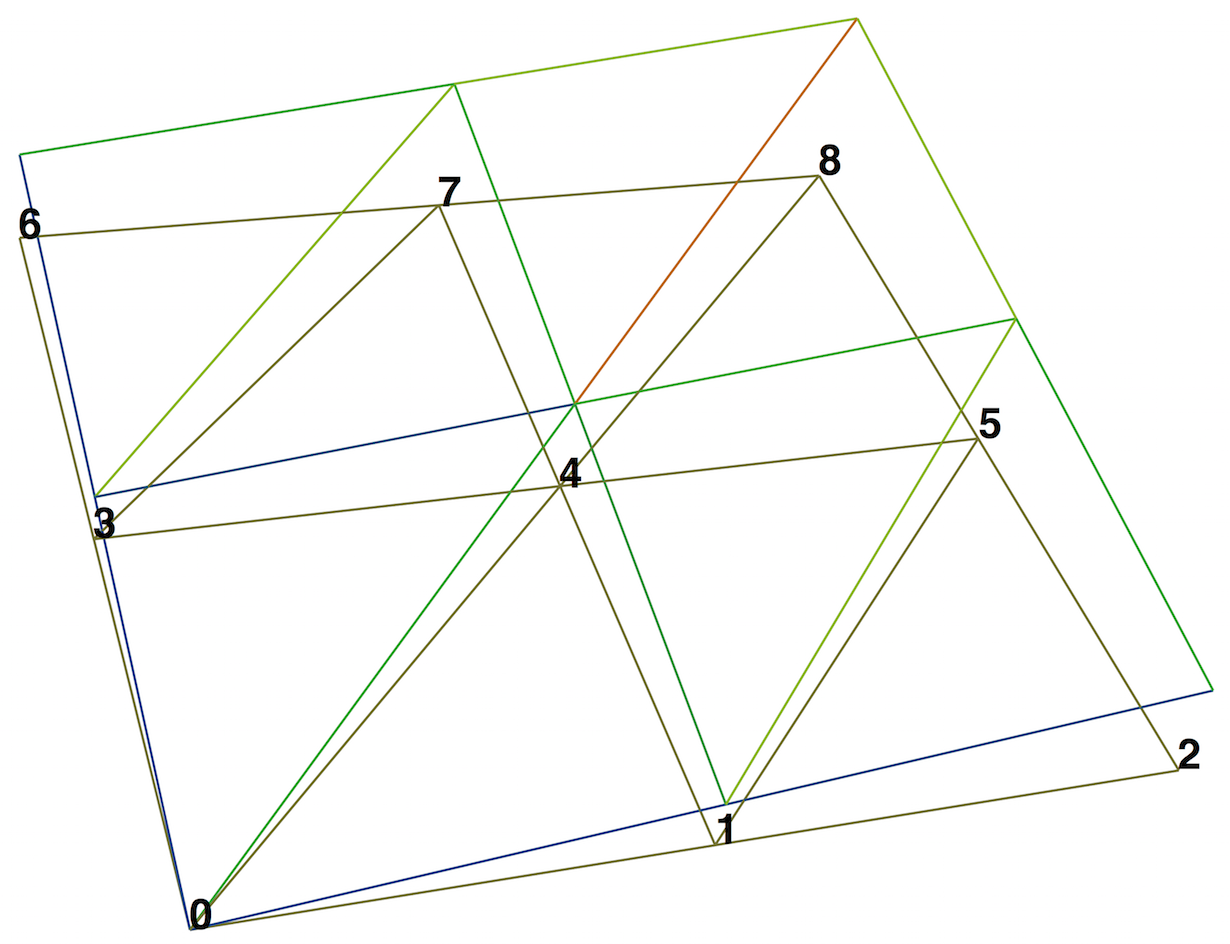
\includegraphics[width=0.75\linewidth]{fig/vertex_numbering.png}}

\vspace{6mm}

\index{vertex values}

我们通过调用来检查值
\verb!u.compute_vertex_values!:

\begin{python}
>>> vertex_values = u.compute_vertex_values()
>>> for i, x in enumerate(coordinates):
...     print('vertex %d: vertex_values[%d] = %g\tu(%s) = %g' %
...           (i, i, vertex_values[i], x, u(x)))
vertex 0: vertex_values[0] = 0          u([ 0.  0.]) = 8.46545e-16
vertex 1: vertex_values[1] = 0.5        u([ 0.5  0. ]) = 0.5
vertex 2: vertex_values[2] = 1          u([ 1.  0.]) = 1
vertex 3: vertex_values[3] = 0.5        u([ 0.   0.5]) = 0.5
vertex 4: vertex_values[4] = 1          u([ 0.5  0.5]) = 1
vertex 5: vertex_values[5] = 1.5        u([ 1.   0.5]) = 1.5
vertex 6: vertex_values[6] = 1          u([ 0.  1.]) = 1
vertex 7: vertex_values[7] = 1.5        u([ 0.5  1. ]) = 1.5
vertex 8: vertex_values[8] = 2          u([ 1.  1.]) = 2
\end{python}

\index{vertex to dof map}
\index{dof to vertex map}

我们可以要求FEniCS给我们从顶点到度数的映射
某个功能空间的自由$V$:

\begin{python}
v2d = vertex_to_dof_map(V)
\end{python}
现在,\verb!nodal_values[v2d[i]]! 会给我们带来的价值
自由
对应于顶点\texttt{i}(\texttt{v2d[i]})。 特别是\verb!nodal_values[v2d]!
是具有相同(顶点编号)顺序的所有元素的数组
作为\texttt{coordinates}。 逆映射,从自由度数到
顶点数由\verb!dof_to_vertex_map(V)!给出。 这意味着
我们可以打电话\verb!coordinates[dof_to_vertex_map(V)]! 得到所有的数组
坐标与自由度相同。 注意
这些映射仅适用于$\mathsf{P}_1$元素的FEniCS。

对于Lagrange度数大于1的元素,有度数
自由度(节点)不对应于顶点。 对于这些
元素,我们可以通过调用获得顶点值
\verb!u.compute_vertex_values(mesh)!,我们可以获得自由度
通过调用\texttt{u.vector()。array()}。 获取坐标相关联
我们需要对所有的自由度进行迭代
网格并要求FEniCS返回与之相关的坐标和自由度
与每个元素(单元格)。 此信息存储在
\texttt{FunctionSpace}的\texttt{FiniteElement}和\texttt{DofMap}对象。该
以下代码说明了如何迭代网格的所有元素
并打印与之相关的坐标和自由度
元件。

\begin{python}
element = V.element()
dofmap = V.dofmap()
for cell in cells(mesh):
    print(element.tabulate_dof_coordinates(cell))
    print(dofmap.cell_dofs(cell.index()))
\end{python}